\newpage
\begin{center}
\noindent\textbf{ГЛАВА 2. ЗАДАЧА ВЫПОЛНИМОСТИ БУЛЕВЫХ ФОРМУЛ И SAT-РЕШАТЕЛИ}\label{chapters:2}
\vspace{1.5mm}
\end{center}

\vspace{5pt}
\textbf{2.1. Определения}\label{chapters:2.1}
\vspace{5pt}

Конъюнктивной нормальной формой (КНФ) называются булева формула вида 
$\Phi_m \left( x_1, x_2, \dots, x_m \right) = D_1 \land D_2 \land \dots \land D_k$,
где каждый дизъюнкт $D_j=t_{j,1} \lor t_{j,2} \lor \dots \lor t_{j,n_j}$, 
и все литералы $t_{j,i}$ – либо переменные, либо их отрицания,
причем переменная может встречаться в дизъюнкте не более одного раза. 
Задача выполнимости КНФ (\textit{ВЫП}, \textit{SAT}) заключается в следующем: для входной формулы $\Phi_m$ указанного вида 
необходимо определить, существует ли набор значений переменных $\left( \alpha_1, \alpha_2, \dots, \alpha_m \right)$ такой,
что $\Phi_m \left( \alpha_1, \alpha_2, \dots, \alpha_m \right) = 1$, выполнима ли $\Phi_m$? 
При этом исследователя часто интересует не только ответ \enquote{да} или \enquote{нет}, но и сам выполняющий набор переменных или доказательство его отсутствия.

Факт принадлежности задачи \textit{ВЫП} к классу $\mathcal{NP}$ является тривиальным. Более содержательное утверждение, 
знаменитая теорема Кука-Левина, открывшее важность этой задачи для теории сложности вычислений, 
а впоследствии и для практических приложений, доказал в 1971 году Стивен Кук (тот же результат независимо получило советский математик Леонид Левин). В работе [\ref{bib:Cook}] он впервые ввел понятие $\mathcal{NP}$-полной задачи и доказал $\mathcal{NP}$-полноту 
задачи выполнимости КНФ, что сделало ее первой известной $\mathcal{NP}$-полной задачей. 
Идея доказательства состоит в построении формулы, которая выполнима тогда и только тогда, когда соответствующая 
недетерминированная машина Тьюринга, решающая выбранную задачу за полиномиальное время, останавливается с положительным ответом.

Этот результат позволил доказать $\mathcal{NP}$-полноту множества других задач путем полиномиального сведения к ним задачи выполнимости КНФ, что стало стандартным способом доказательства $\mathcal{NP}$-полноты. 
Так, в своей работе [\ref{bib:Karp}] 1972 года Ричард Карп доказал $\mathcal{NP}$-полноту $21$ задачи (ныне известных как «список Карпа»), 
среди которых: задача о клике, задача о выполнимости булевых формул с тремя литералами (\textit{3-SAT}, 
для которой известен рандомизированный алгоритм ($\mathcal{PPSZ}$) со сложностью $\mathcal{O} \left( 1.32216n \right)$) [\ref{bib:Rolf}], 
задача о раскраске графа и другие.

Вокруг исследования задачи выполнимости, ее приложений и обобщений сформировалось 
международное научное сообщество \enquote{\textit{SAT Association}}, проводится ежегодная конференция 
\enquote{\textit{International Conference on Theory and Applications of Satisfiability Testing}}, 
публикуется тематический рецензируемый журнал \enquote{\textit{Jour\-nal on Satisfiability, Boolean Modeling and Com\-pu\-ta\-ti\-on, JSAT}}.
Среди перспективных направлений научных исслендований можно отметить изучение задач 
\textit{CSP} (задача удовлетворения ограничений), 
\textit{MAX-SAT} (задача поиска максимального количества выполнимых дизъюнктов), 
\textit{\#SAT} и \textit{ALL-SAT} (подсчет количества выполняющих наборов и их поиск), 
\textit{SMT} (задача выполнимости формул в теориях), 
\textit{QBF} (задача о булевой формуле с кванторной приставкой), 
а также конструирование приближенных ($\mathcal{PTAS}$) и рандомизированных алгоритмов.

Пока вопрос о равенстве классов $\mathcal{P}$ и $\mathcal{NP}$ остается открытым, $\mathcal{NP}$-полнота задачи \textit{SAT} свидетельствует о том, что она является вычислительно сложной и у нас нет эффективных детерминированных алгоритмов, позволяющих в общем случае решать ее за разумное время. С другой стороны, ряд важных прикладных задач естественным образом (например, с помощью преобразования Цейтина) сводится к \textit{SAT} и ее обобщениям: задачи из области автоматизации проектирования (\textit{EDA}), логического синтеза, автоматического доказательства теорем, криптографии, биоинформатики, проверки моделей, формальной верификации программ и автоматического конструирования тестовых покрытий, планирования, построения расписаний.

Интерес исследователей, практическая необходимость, развитие вычислительной техники и новые теоретически результаты привели к созданию ряда подходов (и программных пакетов на их основе – \textit{SAT}-решателей), позволяющих во многих случаях эффективно решать задачу выполнимости. 
Все они так или иначе используют модификации метода направленного перебора и в худшем случае имеют экспоненциальную сложность. Их можно условно разделить на несколько семейств по принципу организации перебора:

\begin{enumerate}[leftmargin=1cm,topsep=0pt,itemsep=-1ex,partopsep=1ex,parsep=1ex,label=\arabic{*}.]

\item
Алгоритмы, основанные на поиске с возвратом, из которых наиболее удачным оказался \textit{DPLL} [\ref{bib:Robinson1962}] и его улучшенный вариант: \textit{CDCL} [\ref{bib:MarquesSilva}] и другие подходы, основанные на методе резолюций.

\item
Вариации генетических алгоритмов, например, \textit{GASAT} [\ref{bib:Lardeux}].

\item
Подходы, основанные на применении машинного и глубокого обучения, например, \textit{NeuroSAT} [\ref{bib:Selsam}], который рассматривает задачу выполнимости как задачу классификации и использует для ее решения рекуррентную нейронную сеть.

\item
Методы стохастического локального поиска [\ref{bib:HoosWalkSAT}], например, \textit{WalkSAT}, базовая идея которого заключается в итеративном выборе по некоторому правилу ложного дизъюнкта и \enquote{переворачивании} одного из входящих в него литералов.

\item
Алгоритмы символьных вычислений, основанные на преобразовании бинарной диаграммы решений и ее обобщениях [\ref{bib:Puri}].

\item
Алгоритмы, основанные на построении набора правил вывода и пошаговом преобразовании формулы в эквивыполнимую [\ref{bib:Puri}].

\end{enumerate}

Современные \textit{SAT}-решатели представляют собой многоуровневые комбинации из нескольких подходов, дополненные различного рода эвристиками (например, случайные рестарты), оптимизациями, преобразованиями формулы [\ref{bib:EénBiere}] (например, исключение переменных методом резолюций или с помощью модифицированной процедуры Фурье-Моцкина) с десятками настраиваемых параметров. Объединение различных техник и тонкая настройка параметров позволяют эффективно решать задачи с тысячами переменных и десятками тысяч дизъюнктов. Отдельного внимания заслуживают детали реализации указанных алгоритмов. Так, мемоизация и специализированные структуры данных могут ускорить выполнение некоторых операций в разы. Другие важные аспекты – возможность инкрементального применения, масштабируемость, эффективное распараллеливание, которое может достигаться несколькими способами: портфельный метод (одновременный запуск нескольких экземпляров решателя); метод \enquote{разделяй и властвуй}, основанный на разбиении формулы на независимые подформулы; параллельный локальный поиск.

Успешность современных алгоритмов при решений индустриальных задач во многом объясняется тем, что они в общем случае имеют регулярную структуру взаимосвязей между переменными. На \figurename{ \ref{chapter1:fig:satgraph}} приведены визуализации индустриальной и случайно сгенерированной задач, полученные методом Clauset-Newman-Moore [\ref{bib:Newsham}].

\begin{figure}[h]
\centering
\captionsetup{justification=centering}
\center{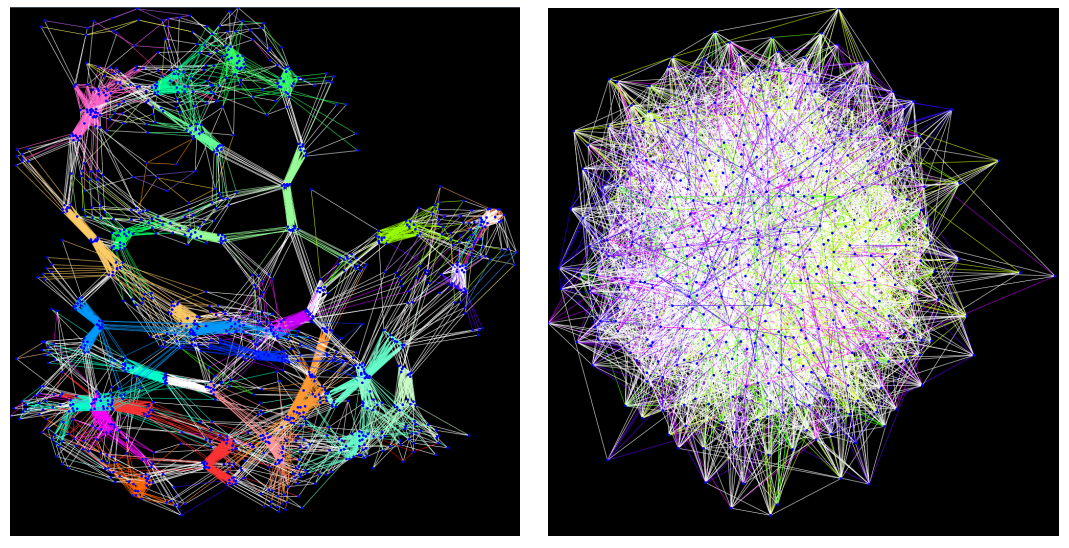
\includegraphics[width=0.7\paperwidth]{chapters/chapter2/sat-graph.png}}
\caption{Сетевая структура индустриальной (слева) и случайно сгенерированной (справа) формул.}
\label{chapter1:fig:satgraph}
\end{figure}

В качестве примера удачной реализации стратегии \enquote{разделяй и властвуй} можно привести проект построения распределенного \textit{SAT}-решателя \textit{SAT@home} [\ref{bib:ZaikinKochemazovSemenov}], выполненного на платформе для GRID-вычислений \textit{BOINC}, реализованный лабораторией Дискретного анализа и прикладной логики Института динамики систем и теории управления СО РАН, позволивший, в числе прочего, найти несколько ортогональных пар диагональных латинских квадратов порядка $10$.

Не все алгоиртмы являются полными в том смысле, что не гарантируют при любом входе завершиться с корректным ответом. Часто отсутствие полноты становится платой за введение дополнитальных эвристик, которые могут значительно ускорить решение задач некоторого класса. 
Многие реализации алгоритма \textit{CDCL} в случае невыполнимости КНФ позволяют построить \enquote{сертификат невыполнимости} в одном из общепринятых форматов (\textit{TraceCheck}, \textit{DRUP} [\ref{bib:HeuleBiere}]), которое можно верифицировать специальной утилитой, человеку это сделать обычно не под силу. 
Так, группе ученых во главе с Марином Хойле удалось с помощью \textit{SAT}-решателя и суперкомпьютера \textit{Stampede} ($800$ ядер) построить доказательство в формате \textit{DRAT} отсутствия такой двухцветной раскраски множества $\{1, \dots, 7825\}$, при которой ни одна пифагорова тройка из этого множества не является одноцветной (булева проблема пифагоровых троек) [\ref{bib:HeuleKullmann}]. 
Размер файла с доказательством достиг $200$ терабайт. Такой метод доказательства утверждений используется все чаще, хотя и не приветствуется математическим сообществом.

\begin{figure}[h]
\centering
\captionsetup{justification=centering}
\center{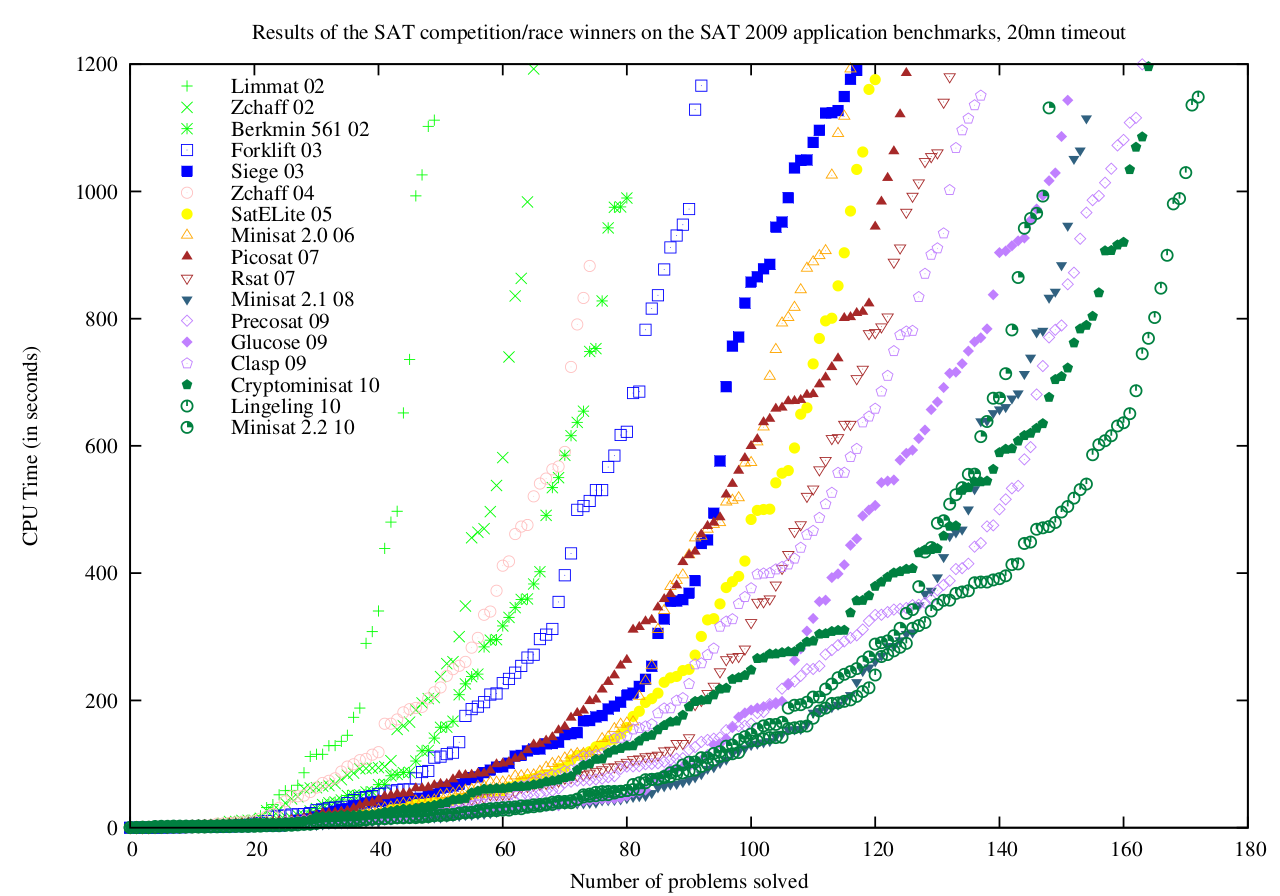
\includegraphics{chapters/chapter2/sat-competition.png}}
\caption{Результаты The International SAT Competition 2009 года.}
\label{chapter1:fig:satcomp}
\end{figure}

На протяжении двух десятков лет проводятся международные состязания по решению задачи \textit{SAT} 
[\ref{bib:Järvisalo}, \ref{bib:BiereCadical}], на которых участники соревнуются в скорости решения специально подобранных задач, записанных в стандартном формате \textit{DIMACS}, при различных условиях (последовательные, параллельные вычисления) и ограничениях. Построение коротких и \enquote{сложных} конкурсных задач, а также формализация свойств формулы, которые делают ее сложной для \enquote{SAT}-решателя – отдельная интересная проблема. Результаты соревнования 
(\figurename{ \ref{chapter1:fig:satcomp}}) публикуются на сайте \url{http://www.satcompetition.org/}. Победителями этого соревнования в разные годы становились \textit{MiniSAT}, \textit{Glucose}, \textit{Lingeling}, \textit{CryptoMiniSat}, \textit{YalSAT}, \textit{MapleSAT}, \textit{abcdSAT}, \textit{RISS}. Все эти проекты имеют открытый исходный код и доступны для свободного использования. Отметим, что победителями последних на данный момент сореванований \textit{SAT Race 2019} стал \textit{SAT}-решатель \textit{MapleLCMDiscChronoBT-DL}, предложенный
командой ИДСТУ СО РАН (С. Кочемазов, О. Заикин и др.) [\ref{bib:HeuleSATRace2019},\ref{bib:Kochemazov}]. 
Группа ученых из Университета Британской Колумбии поддерживает коллекцию \textit{SAT}-задач различного уровня сложности, известную как бенчмарк \textit{SATLIB} 
[\ref{bib:HoosStützle}]. На протяжении многих лет наилучшие результаты на таких соревнованиях, а также и при решении практических задач, показывают алгоритмы, базирующиеся на идее \textit{CDCL}, о который и пойдет речь далее в этой главе.

\vspace{5pt}
\textbf{2.2. Алгоритм DPLL}\label{chapters:2.2}
\vspace{5pt}

Алгоритма \textit{DPLL} [\ref{bib:Robinson1962}] – это полный и высокоэффективный алгоритм решения задачи выполнимости, основанный на классическом алгоритме решения задач комбинаторной оптимизации: поиск в глубину с возвратом. Он назван в честь своих авторов: Дэвиса, Патнема, Логемана, Лавленда, впервые опубликован в 1962 году и является усовершенствованной версией \textit{DP}, предыдущего алгоритма Дэвиса и Патнема, основанного на методу резолюций.

Далее введем несколько общепринятых в литературе обозначений. 
Поскольку порядок элементов не важен, здесь и далее формулу $\Phi$ удобно представлять как множество дизъюнктов $\{ D_1, \dots, D_k \}$, 
каждый из которых является множеством литералов $\{ t_{j,1}, \dots ,t_{j,n_j} \}$ над переменными из множества $X$. Если множество дизъюнктов пусто, формула считается тривиально выполнимой, если один из дизъюнктов пуст - не выполнимой.
В контексте алгоритмов поиска выполняющих наборов каждая переменная $x \in  X$ может находиться в разных состояниях. Переменной может быть присвоено значение $\nu(x)$, $\nu: X \mapsto \{ 0, 1, ?\}$, где знаком \enquote{$?$} обозначается, что значение переменной не определено. Если $\forall x \in X $ $\nu(x) \in \{ 0, 1\}$, то присваивание называется \textit{полным}, иначе - \textit{частичным}. Присваивание $\nu$ позволяет вычислить значения литерала $l^{\nu}$, дизъюнкта $D^{\nu}$ и всей формулы $\Phi^{\nu}$, в этом случае говорят, что им присвоено соответствующее значение. Переменная называется \textit{чистой}, 
если она входит в формулу либо только с отрицанием, либо только без отрицания. \textit{Чистую} переменную (и все ее дизъюнкты) можно удалить из формулы, не нарушив ее выполнимость, такая операция называется \textit{удаление чистых переменных}. 

В ходе вычислений каждый дизъюнкт, в зависимости от функции присваивания, можно охарактеризовать одним из четырех состояний: \textit{невыполненный}, \textit{выполненный}, \textit{единичный}, \textit{неопределенный}. Дизюнкт называется невыполненным, если всем его литералам присвоен $0$, выполненным, если хотя бы одному из его литералов присвоено значение $1$, единичным, если всем литералам, кроме одного, значение которого не определено, присвоено значение $1$, в остальных случаях дизюнкт считается неопределенным. Конечная цель алгоритма - сделать все дизъюнкты выполненными путем присваивания переменным значений.

Ключевой процедурой алгоритма \textit{DPLL} является \textit{разрешение булевых ограничений}. 
Если на каком-то этапе вычислений в формуле появился единичный дизъюнкт, то сделать его выполненным можно только одним способом: выбрать подходящее значение неопределеной переменной, которое называется \textit{предполагаемым}. На этом этапе возможен \textit{конфликт}: 
два разных дизъюнкта могут \enquote{потребовать} одновременно противоположных значений переменной. Единичный дизъюнкт $\omega$, 
который был использован для вывода предполагаемого значения переменной $x$, называется ее \enquote{антецедентом}: $\omega = \alpha(x)$. 
Если переменная $x$ получила свое значение в результате присваивания, полагают $\alpha(x) = NIL$.
В ситуации конфликта, присваивания, которые послужили причиной конфликта, отменяются, алгоритм возвращается на шаг назад. 
Базовый алгоритм является рекурсивным, поэтому можно ввести понятие \textit{уровня присваивания} переменной $\delta(x)$, который равень уровню рекурсии, на котором было выполнено присваивание. Для неопределенных переменных $\delta(x_i)=-1$, для предполагаемых 
$\delta(x_i) = \max \{ \{0\} \cup \{ \delta(x_j): x_j \in \alpha(x_i) \land x_j \ne x_i \} \}$. 
Обозначения $x = v @ d$, $d/x=v$ эквивалентны $\delta(x) = d$ и $\nu(x) = v$. 
На практике разрешение булевых ограничений приводит к каскадному сокращению формулы. 

Основная схема алгоритма: по некоторому правилу выбрать из множества неопределенных переменных \textit{переменную ветвления}, присвоить ей некоторое значение, сохранить его в \textit{стеке присваиваний}, преобразовать формулу. Затем рекурсивно проверяется выполнимость новой формулы: если она выполнима, то и исходная формула была выполнимой, алгоритм завершает работу с результатом \textit{SAT}, в противном случае (обнаружен конфликт) запустить ту же процедуру, используя противоположное значение переменной. 
Если оба значения выбранной переменной привели к конфликту, алгоритм возвращется на шаг назад, выталкивая одно присваивание из стека. Если возвращаться \enquote{некуда}, алгоритм выдает \textit{UNSAT}. 
В общем случае алгоритм завершает работу с результатом \textit{UNSAT}, если был выполнен полный перебор всевозможных комбинаций значений переменных.

Преобразование формулы состоит из следующих шагов:
\begin{enumerate}[leftmargin=1cm,topsep=0pt,itemsep=-1ex,partopsep=1ex,parsep=1ex,label=\arabic{*}.]
\item
Из формулы удаляются все дизъюнкты, которые стали выполненными после присваивания переменной, 
все остальные вхождения этой переменной удаляются.
\item Выполняется разрешение булевых ограничений.
\item Выполняется удаление чистых переменных.
\end{enumerate}

Псевдокод алгоритма можно записать следующим образом:

\definecolor{codegreen}{rgb}{0,0.6,0}
\definecolor{codegray}{rgb}{0.5,0.5,0.5}
\definecolor{codepurple}{rgb}{0.58,0,0.82}
\definecolor{backcolour}{rgb}{0.95,0.95,0.92}

\lstdefinestyle{mystyle}{    
    keywordstyle=\color{magenta},
    commentstyle=\color{codegreen},
    lineskip=1ex,
    numberstyle=\tiny\color{codegray},
    stringstyle=\color{codepurple},
    basicstyle=\ttfamily\small,
    breakatwhitespace=false,         
    breaklines=true,                 
    captionpos=b,                    
    keepspaces=true,                 
    numbers=left,                    
    numbersep=5pt,                  
    showspaces=false,                
    showstringspaces=false,
    showtabs=false,                  
    tabsize=2
}

\lstset{style=mystyle}

\lstset{xleftmargin=1.5cm,frame=tlbr,framesep=8pt,framerule=0pt}

\begin{lstlisting}[language=Python, mathescape=true]
def DPLL($\Phi$):	
	$\Phi$ = preprocess($\Phi$)
 	$\Phi$ = pure_literal_elimination($\Phi$)
 	$\Phi$ = unit_propagation($\Phi$)	
	if $\Phi=\{\}$:
		return SAT
	if $\{\} \in \Phi$:
		return UNSAT
 	x = choose_literal($\Phi$)
	return DPLL($\Phi \land \{x\}$) or DPLL($\Phi \land \{\overline{x}\}$)
\end{lstlisting}

\vspace{5pt}

Доработка этого алгоритма ведется в нескольких направлениях:

\begin{enumerate}[leftmargin=1cm,topsep=0pt,itemsep=-1ex,partopsep=1ex,parsep=1ex,label=\arabic{*}.]
\item Построение различных эвристических правил выбора переменной ветвления и соответствующего литерала.
\item Построение ленивых структур данных, позволяющих ускорить отдельные шаги вычисления и сократить объем используемой памяти.
\item Использование \enquote{нехронологических} возвратов и \enquote{запоминание} конфликтных дизъюнктов. 
\end{enumerate}

Последняя идея привела к созданию алгоритма \textit{CDCL}, который является ядром практически всех современных \textit{SAT}-решателей.

\vspace{5pt}
\textbf{2.3. Алгоритм CDCL}\label{chapters:2.3}
\vspace{5pt}

Алгоритм \textit{CDCL} [\ref{bib:BiereHeule}] (Conflict-Driven Clause Learning – \enquote{обучение дизъюнктам, управляемое конфликтами}) предложен в 1996 году независимо двумя группами исследователей. К уже известным шагам \textit{DPLL} добавляется построение \textit{имликационного графа}, который позволяет выводить и \enquote{запоминать} зависимости между переменными в виде новых дизъюнктов. Такой анализ структуры конфликтов резко сокращает пространство поиска, ускоряет процесс вычисления, дает возможность \enquote{не натыкаться} на одни и те же конфликты, а также, в случае невыполнимости, строить более краткие доказательства. В случае конфликта импликационный граф позволяет понять, какие присваивания к нему привели, что открывает возможность \enquote{нехронологических} возвратов: возврат к тому уровню рекурсии, который послужил причиной конфликта. Кроме того, этот метод дает некоторые ключи к построению инкрементальных и распределенных \textit{SAT}-решателей: обмен \enquote{выученными} дизъюнктами между параллельными процессами оказывается гораздо эффективнее простых портфельных методов.

Импликационный граф представляет собой ориентированный ациклический граф $I = \left(V_I, E_I \right)$. 
Его вершины соответствуют присваиваниям, одна специальная вершина $\kappa$ обозначает ситуацию конфликта: $V_I \subseteq X \cup \{ \kappa \} $.
Ребра графа соответствуют андецедентам переменных. 
Для формального определения ребер введем предикат $\lambda(z, \omega)$ вхождения переменной $z$ в дизъюнкт $\omega$:
\begin{equation*}
\lambda(z, \omega) = 
\begin{cases}
1 & \text{если } z \in \omega \lor \overline{z} \in \omega \\
0 & \text{иначе}
\end{cases}
\end{equation*}
Предикат $\nu_0(z, \omega)$ принимает значение $1$ тогда и только тогда, когда $z$ входит в $\omega$ и равен $0$:
\begin{equation*}
\nu_0(z, \omega) = 
\begin{cases}
1 & \text{если } \lambda(z, \omega) \land z \in \omega \land \nu(z) = 0 \\
1 & \text{если } \lambda(z, \omega) \land \overline{z} \in \omega \land \nu(z) = 1 \\
0 & \text{иначе}
\end{cases}
\end{equation*}
Аналогично,
\begin{equation*}
\nu_1(z, \omega) = 
\begin{cases}
1 & \text{если } \lambda(z, \omega) \land z \in \omega \land \nu(z) = 1 \\
1 & \text{если } \lambda(z, \omega) \land \overline{z} \in \omega \land \nu(z) = 0 \\
0 & \text{иначе}
\end{cases}
\end{equation*}
Наконец, $(z_1, z_2) \in E_I$, если следующий предикат равен $1$:
\begin{equation*}
\epsilon(z_1, z_2) = 
\begin{cases}
1 & \text{если } z_2 = \kappa \land \lambda(z_1, \alpha(\kappa)) \\
1 & \text{если } z_2 \ne \kappa \land \alpha(z_2)=\omega \land \nu_0(z_1, \omega) \land \nu_1(z_2, \omega) \\
0 & \text{иначе}
\end{cases}
\end{equation*}
Таким образом, множество ребер графа импликации $I$ можно определить как $V_I = \{ (z_1, z_2): \epsilon(z_1, z_2) = 1\}$. Наконец, каждое ребро $(z_1, z_2) \in E_I$ помечается как $\iota(z_1, z_2) = \alpha(z_2)$.


На \figurename{ \ref{chapter1:fig:impgraph}} приведен пример импликационного графа для формулы 
$$
\varphi = \omega_1 \land \omega_2 \land \omega_3 = 
\left(x_1 \lor x_{31} \lor \overline{x_2} \right)
\land
\left(x_1 \lor \overline{x_3} \right)
\land
\left(x_2 \lor x_3 \lor x_4 \right)
$$
и присваиваний $x_{31} = 0@3$, $x_1 = 0@5$.

\begin{figure}[h]
\centering
\captionsetup{justification=centering}
\center{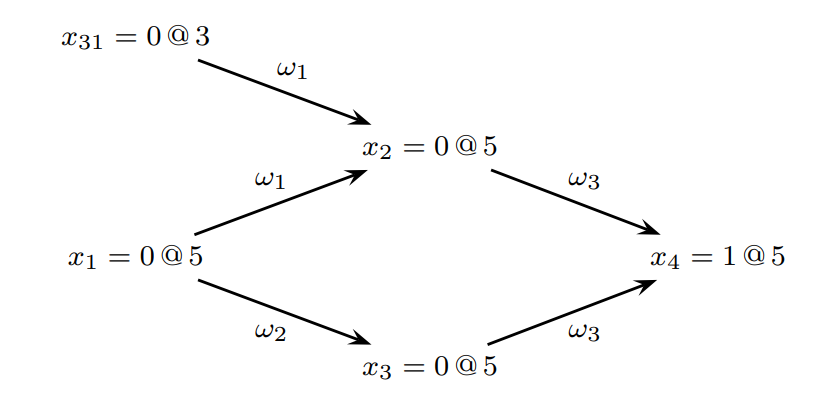
\includegraphics[width=0.5\paperwidth]{chapters/chapter2/imp-graph.png}}
\caption{Пример импликационного графа.}
\label{chapter1:fig:impgraph}
\end{figure}

Псевдокод алгоритма \textit{СDCL} можно записать следующим образом:

\begin{lstlisting}[language=Python, mathescape=true]
def CDCL($\varphi$, $\nu$):	
	if UnitPropagation($\varphi$, $\nu$) == CONFLICT:
		return UNSAT
	dl = 0 # decision level
	while not AllVariablesAssigned($\varphi$, $\nu$):
		($x$, $v$) = PickBranchingVariable($\varphi$, $\nu$)
		dl = dl + 1
		$\nu$ = $\nu \cup \{ (x, v) \}$
		if UnitPropagation($\varphi$, $\nu$) == CONFLICT:
			$\beta$ = ConflictAnalysis($\varphi$, $\nu$)
			if $\beta < 0$:
				return UNSAT
			else:
				Backtrack($\varphi$, $\nu$, $\beta$)
				dl = $\beta$
	return SAT
\end{lstlisting}

К уже известным шагам алгоритма \textit{DPLL} добавлена операция \textit{анализа конфликта}. 
Эта процедура вычисляет уровень возврата и новую дизъюнкцию. Анализ конфликта состоит в последовательном проходе по графу импликации от вершины $\kappa$ к антецедентам в сторону уменьшения уровня присваивания и применении правила резолюции (обозначим как $\odot$), что на каждом шаге порождает новую дизъюнкцию. Более формально, определим предикат $\xi(\omega, l, d)$, который равен $1$, если в дизъюнкт $\omega$ входит предполагаемый лиретал $l$, который получил свое значение на уровне $d$:
\begin{equation*}
\xi(\omega, l, d) = 
\begin{cases}
1 & l \in \omega \land \delta(l) = d \land \alpha(l) \ne NIL \\
0 & \text{иначе}
\end{cases}
\end{equation*}
Тогда промежуточные дизъюнкты $\omega_{L}^{d,i}$, полученные после применения $i=0,1,2,...$ резолюций можно определеить следующим образом:
\begin{equation*}
\omega_{L}^{d,i} = 
\begin{cases}
\alpha(\kappa) & \text{если } i = 0 \\
\omega_{L}^{d,i-1} \odot \alpha(l) & \text{если } i \ne 0 \land \xi(\omega_{L}^{d,i-1}, l, d) = 1 \\
\omega_{L}^{d,i-1} & \text{если } i \ne 0 \land \forall l \, \xi(\omega_{L}^{d,i-1}, l, d) = 0
\end{cases}
\end{equation*}

На шаге $i$, при котором $\omega_{L}^{d,i} = \omega_{L}^{d,i-1}$, процесс заканчивается и $\omega_{L} \triangleq \omega_{L}^{d,i}$ представляет новый \enquote{выученную} дизъюнкт, который добавляется к уже известным.
Отметим, что этот процесс очень близко связан с поиском разреза графа импликации. В современных \textit{SAT}-решателях используются ряд дополнительных приемов (\textit{Learned clauses minimization}) для сокращения выученного дизъюнкта [\ref{bib:BiereHeule}], и, как правило, используют немного модифицированный подход \textit{1-UIP}, который сводится к поиску первого доминатора импликационного графа, выполняется за линейное время и гарантирует некоторые полезные свойства для выученной дизъюнкции.

\vspace{5pt}
\textbf{2.4. Детали реализации современных SAT-решателей}\label{chapters:2.4}
\vspace{5pt}

В этом разделе рассатриваются некоторые технические аспекты реализации \textit{SAT}-решателей, такие как экристики ветвления, случайные рестарты, наблюдаемые литералы, структура данных, методы подбора параметров, которые сыграли ключевую роль [\ref{bib:Katebi}] в успешности современных алгоритмов. Стоит отметить, что это далеко не исчерпывающий список приемов и их всестороннему исследованию посвящено множество работ.

\textbf{Эвристики ветвления}

\textit{Эвристикой ветвления} называется алгоритм выбора переменной ветвления. Простейший способ, в данном случае, - случайный выбор. Еще один возможный вариант - выбирать ту переменную, присваивание которой порождает как можно больше единичных дизъюнктов.
Парадоксально, но случайный выбор нередко позволяет получить результат быстрее прочих, поэтому все эвристики так или иначе включают элемент случайности. 
С другой стороны, в ходе вычислений решатель накапливает определенную информацию, которую можно использовать при выборе переменной ветвления для того, чтобы ускорить вычислительный процесс, сделать его более направленным и контролируемым, а не полагаться на волю случая. 

В литературе предложен ряд эффективных методов, которые используют динамическую информацию о ходе вычислений, 
структуре конфликтов [\ref{bib:MarquesSilva1999}], имеют некоторые теоретические обоснования и широко используются на практике. 
Ключевая идея: каким-либо образом оценить \enquote{важность} переменной, используя имеющиеся данные. Стоит отметить, что вычисление такой характеристики может быть достаточно \enquote{дорогим}, поэтому нередко умозрительно удачные, но \enquote{тяжелые} подходы проигрывают на практике. Далее рассматривается несколько наиболее популярных методов.

На случайно сгенерированных задачах лучшие результаты показывает эвристика, предложенная \textbf{Bohm}: на каждом шаге из множества неопредленных переменных выбирается переменная с максимальным значением вектора 
$H_i(x_i) = \left(H_1(x_i), \dots, H_m(x_i)\right)$ 
(в смысле лексикографического порядка), где
$H(x) = \alpha \max \{ h_i(x), h_i(\overline{x}) \} + \beta \min \{ h_i(x), h_i(\overline{x}) \}$
и $h_i(x)$ – количество неопределенных дизъюнктов с $i$ литералами, содержащих $x$.
Такая эвристика стремится сделать истинными короткие дизъюнкты (при $x=1$) либо их уменьшить.

Метод \textbf{MOM} (\textit{Maximum Occurrences on Minimum sized clauses}) предлагает выбирать переменную $x$, которая максимизирует функцию 
$S(x) = \left(f^{*}(x) + f^{*}(\overline{x})\right) \cdot 2^{k} + f^{*}(x) \cdot f^{*}(\overline{x})$, где $f^{*}(l)$ - это количество вхождений литерала $l$ в невыполненные дизъюнкты минимального размера. Этот метод выделяет переменные, которые входят в большое количество коротких дизъюнкций с отрицанием или без (при достаточно большом $k$) и одновременно.

Эвристика \textbf{Jeroslow-Wang} устроена следующим образом. Для литерала $l$ вычисляется $J(l) = \sum_{D \in \Phi} 2^{-\left|D\right|}$
Односторонний вариант \textbf{JW-OS} предполагает выбор литерала $l$ с наибольшим значением $J(l)$. Двусторонний \textbf{JW-TS} – поиск переменной $x$ с наибольшей суммой $J(x)+J(\overline{x})$ и присваивание ей $1$, если $J(x) \ge J(\overline{x})$. Такой метод стремится выбирать переменные, которые часто встречаются в коротких дизъюнктах.

\textbf{Эвристики подсчета литералов} устроены значительно проще предыдущих и имеют очевидный интуитивный смысл. Пусть $C_p(x)$ - количество неопределенных дизъюнкций, в которые $x$ входит без отрицания, $C_n(x)$ - с отрицанием. 
Характеристики $C_p(x)$ и $C_n(x)$ можно учитывать в сумме или по отдельности:

\begin{enumerate}[leftmargin=1cm,topsep=0pt,itemsep=-1ex,partopsep=1ex,parsep=1ex,label=\arabic{*}.]
\item Выбрать $x$, для которого $C_p(x) + C_n(x)$ максимальна (\textbf{DLCS}) и присваиванить ей $1$, если $C_p(x) \ge C_n(x)$.
\item Выбрать $x$, для которого $C_p(x)$ ($C_n(x)$) максимальна (\textbf{DLIS}) и присвоить ей заналогично предыдущему пункту (\textbf{DLIS}) или случайно (\textbf{RDLIS}).
\end{enumerate}

Характеристика \textbf{VSIDS} (\textit{Variable State Independent Decaying Sum}) основана на анализе конфликтов и вычисляется инкрементально:

\begin{enumerate}[leftmargin=1cm,topsep=0pt,itemsep=-1ex,partopsep=1ex,parsep=1ex,label=\arabic{*}.]
\item На старте каждым литералом ассоциируется счетчик с нулевым значением.
\item При добавлении очередной \enquote{выученной} дизъюнкции счетчик, ассоциированный с каждым литералом из этой дизъюнкции, увеличивается на $1$.
\item С некоторым периодом все счетчики делятся на константу.
\end{enumerate}

На шаге ветвления выбирается литерал с наибольшим значением счетчика (случайно в случае ничьей). Такая эвристика стремится удовлетворить последние конфликтные дизъюнкты и направляет процесс поиска в сторону их разрешения, что может быть особенно эффективно при решении сложных задач (например, задач с функциональными зависимостями между переменными, в которых конфликты возникают часто). Ее подсчет достаточно прост с вычислительной точки зрения: счетчики обновляются только в случае конфликта.

Метод \textbf{LEFV} (\textit{Last Encountered Free Variable}) очень быстр и хорошо подходит для невыполнимых формул: запоминается неопределенная переменная, которую алгоритм \enquote{встретил} последней на этапе разрешения булевых ограничений. На этапе ветвления выбирается отмеченная переменная, если ее значение все еще не определено, иначе - случайная.

В \textit{MapleCOMSPS} [\ref{bib:Liang}] предложен метод численной оценки \textbf{learning rate} - вероятности того, 
что литерал $v$ породит конфликтный дизъюнкт ($LR(v) = \frac{P(v,I)}{L(I)}$) 
методом обучения с подкреплением (\enquote{многорукий бандит}), где 
$I$ - интервал времени между присваиванием $v$ и возвратом его к неопределенному состоянию, 
$P(v,I)$ - количество выученных дизъюнктов, в которых $v$ задействован на интервале $I$,
$L(I)$ - общее количество выученных дизъюнктов на интервале $I$. Максимизация этой оценки ведет к выбору переменной, которая устраняет как можно больше конфликтов.

После выбора переменной ветвления необходимо присвоить ей значение, которое также можно выбирать разными способами. В \textit{MiniSAT} переменной ветвления в первую очередь присваивается $0$. В \textit{Rsat} предложен метод \enquote{запоминания фазы}: переменной с некоторой вероятностью присваивается значение, которое было получено последним в ходе разрешения булевых органичений.

\textbf{Рестарты}

Частые случайные рестарты широко используются при решении задач комбинаторной оптимизации, помогают бороться с проблемой \enquote{тяжелых} хвостов [16]. Под рестартом подразумевается перезапуск алгоритма в некоторый момент, определяемый политикой рестартов. При этом часть информации, накопленной на предыдущем шаге, можно сохранить: выученные дизъюнкции, статистики, накопленные при выборе переменных ветвлений, другая информация о структуре формулы. Было показано, что при переносе одной выученной дизъюнкции и выполнении некоторых других слабых условий полнота алгоритма сохраняется [\ref{bib:Kullmann2009}]. Рестарты во многих случаях приводят к построению более кратких доказательств невыполнимости.

Перезапуск алгоритма позволяет ему \enquote{не застревать} в локальном подпространстве решений. Элемент случайности при выборе переменной ветвления позволяет продолжить поиск в новом направлении. Эффективность этого метода можно объяснить следующим образом: накопленные в ходе вычислений данные отражают текущее представление решателя о том, в каком порядке необходимо выбирать переменные. При этом в отсутствие рестарта решатель не может полностью их использовать, так как ограничен принятыми ранее решениями.

Принятие решения о рестарте, как правило, основывается на количестве конфликтов, наблюдаемых в текущем запуске: 
оно ограничивается некоторым растущим рядом. В качестве такого ряда используются [\ref{bib:Kullmann2009}] арифметические прогрессии (\textit{zChaff}), геометрические прогрессии (\textit{MiniSat}), ряд Луби (\textit{MiniSat}) вида $u * t_i$, где $u$ - числовой параметр и 
\begin{equation*}
t_i = 
\begin{cases}
2^{k-1} & i = 2^k - 1 \\
t_{i - 2^{k-1} + 1} & 2^{k-1} \leq i < 2^k - 1 \\
\end{cases}
\end{equation*}

\textbf{Удаление дизъюнктов}

Неконтролируемое добавление \enquote{выученных} дизъюнктов может привести к разрастанию формулы и снизить эффективность всех остальных операций. Поэтому были предложены методы оценки дизъюнктов, который позволяют выбирать в каком-то смысле самые \enquote{полезные} из них. 
Так, в \textit{Glucose} был предложен метод \textit{Literals Blocks Distance (LBD)} [\ref{bib:Audemard}]: 
выученный дизъюнкт разбивается на блоки литералов с одинаковым уровнями присваиваний, 
характеристика \textit{LBD} полагается равной количеству блоков. Дизъюнкты, для которых $LBD=2$ перманентно добавляются к формуле. 
В \textit{MapleLCMDistChronoBT-DL} [\ref{bib:Kochemazov}] перманентно сохраняются многократно встречающиеся конфликтные дизъюнкты.  
Кроме того, применяются некоторые параметрические пороги, при превышении которых \enquote{выученные} дизъюнкты удаляются:

\begin{enumerate}[leftmargin=1cm,topsep=0pt,itemsep=-1ex,partopsep=1ex,parsep=1ex,label=\arabic{*}.]

\item Запоминаются дизъюнкты, содержащие не более $n$ литералов.

\item Запоминаются дизъюнкты, содержащие не более $n$ неопределенных литералов.

\item Запоминаются дизъюнкты, содержащие не более $n$ литералов или не более $1$ неопределенного литерала.

\end{enumerate}

\textbf{Наблюдаемые литералы}

По некоторым оценкам, эффективные реализации SAT-решателей тратят до $90\%$ времени на процедуру разрешения булевых ограничений. Наблюдение за литералами позволяет драматически ускорить этот процесс. Предположим, что на очередном шаге была выбрана некоторая переменная ветвления и ее значение. Далее необходимо найти все невыполненные дизъюнкты, в которых остался ровно один неопределенный литерал. Последовательное сканирование формулы на каждой итерации не эффективно, поэтому в [\ref{bib:Moskewicz}] был предложен метод наблюдения за двумя литералами.

В каждом дизъюнкте отмечается два любых неложных литерала. Очевидно, что до тех пор, пока один из наблюдаемых литералов не стал ложным, данная дизъюнкция не является единичной. Таким образом, к этой дизъюнкции необходимо обращаться только тогда, когда одному из наблюдаемых литералов присвоен $0$. Возможны два случая:

\begin{enumerate}[leftmargin=1cm,topsep=0pt,itemsep=-1ex,partopsep=1ex,parsep=1ex,label=\arabic{*}.]

\item Дизъюнкт не является единичным, то есть все еще содержит как минимум два неложных литерала, один из которых – наблюдаемый, а другим можно заменить прежний наблюдаемый литерал, поддерживая инвариант: в каждой невыполненной дизъюнкции отмечены два неложных литерала.

\item Дизъюнкт стал единичным. Тогда значение второго наблюдаемого литерала выводится и дизъюнкт помечается как выполненный.

\end{enumerate}

Таким образом сокращается количество обращений к памяти, при этом откат на шаг назад по дереву рекурсии не требует \enquote{перевыбора} наблюдаемых литералов. Отмечают, что при корректном управлении памятью этот подход позволяет ускорить и присваивание за счет сокращения количества промахов кэша процессора.

\textbf{Структуры данных и управление памятью}

Базовые структура данных, которыми оперирует \textit{SAT}-решатель – это множество объектов, представляющих литералы, список дизъюнктов, где каждый элемент представляет собой массив ссылок на свои литералы и словарь, где ключом является переменная, а значением – два списка дизъюнктов, в которые переменная входит с отрицанием и без. Позднее были предложены [\ref{bib:Nadel2002}] списки дизъюнктов типа \textit{Head and Tail}, где для каждой дизъюнкции поддерживается два указателя, которые на старте указывают на первый и последний литералы, по ходу вычислений сдвигаются навстречу друг другу, что позволяет ускорить отмену присваивания и поиск единичных дизъюнктов, и \textit{WLCC}, в котором кроме двух ссылок внутри каждой дизъюнкции литералы сортируются по возрастанию уровня присваивания.

Интенсивное добавление и удаление дизъюнкций требует специального обращения с оперативной памятью. Поскольку операции динамического запроса памяти у операционной системы (\textit{malloc} и аналоги) является относительно \enquote{дорогими}, многие реализации используют свою собственную, и, как правило, ленивую, схему управления памятью, основанную на пулах объектов, списках свободной памяти, кешировании и периодической сборке мусора. При запуске у системы запрашивается блок памяти достаточно большого размера, в котором размещаются объекты. При удалении они помечаются специальным флагом. Периодически производится операция сборки мусора, помеченные объекты физически удаляются из памяти.

Де-факто стандартом при разработке продобных систем стал язык программирования C\texttt{++} и операционные системы семейства UNIX.
C\texttt{++} позволяет, с одной стороны, описать достаточно высокоуровневые абстракции, с другой – контролировать процессы выделения и освобождения памяти на низком уровне. Так, одна из наиболее идиоматичных реализаций \textit{SAT}-решателя – \textit{MiniSat} – реализована на C\texttt{++} [\ref{bib:Sorensson}]. Авторы, используя метапрограммирование и шаблоны, имплементировали эффективные примитивы, структуры данных, и удобный программный пользовательский интерфейс (\textit{API}). В данный момент почти каждый новый проект, будь то попытка ввести дополнительную эвристику или принципиально новая конструкция алгоритма, основывается на \textit{MiniSat}. Как правило, предполагается, что \textit{SAT}-решатель будет испрользоваться через интерфейс командной строки, куда также выводится оперативная информация о ходе решения. Стоит также отметить библиотеку-\enquote{обертку} \textit{python-sat}, автор которой построил унифицированный программный интерфейс на языке \textit{Python}, предоставляющий примитивы для сохранения, загрузки, генерации, обработки формул и единообразного вызова более $10$ \textit{SAT}-решателей.

\textbf{Выбора стратегии решения}

В современных SAT-решателях, как правило, используется широкий набор политик, контролирующих ход решения задачи. Они параметризуются набором числовых и категориальных параметров. Все вместе – набор эвристик и их параметры – называются стратегией решения. В работе [22] была сделана попытка статистически оценить, какие из техник вносят наибольший вклад в \enquote{успех} алгоритма путем их последовательного отключения и сравнения результатов. Авторы пришли к выводу, что выбор стратегии решения зависит от конкретной задачи и в общем случае не удается дать каких-либо надежных рекомендаций. Почти все реализации поставляются с встроенным набором стратегий, подобранным авторами, 
например, в \textit{CryptoMiniSat} их около $20$. Если встроенная стратегия оказалась неудачной, исследователь может подобрать параметры вручную, что оказывается отдельной непростой задачей: в эффективном \textit{SAT}-решателе \textit{lingeling} их около 30.

В \textit{SATzilla} [\ref{bib:SATzilla}] предложен неожиданный подход решения проблемы выбора стратегии решения, который основывается на предположении, что для формул, кодирующих задачи из одной области, или близких в смысле некоторой метрики, можно использовать сходные стратегии. Точнее, авторы предлагают рассматривать задачу выбора стратегии как задачу классификации, где объекты – это формулы, а метки классов – стратегии, и решать ее методом $k$-ближайших соседей. При удачном выборе метрик и подходящей обучающей выборке (ее можно построить на основе бенчмарка \textit{SATLIB}, в котором представлены задачи из целого ряда областей), такой метод автоматического выбора параметров выигрывает у жестких предопределенных стратегий, что доказывают результаты \textit{SAT Competition} [\ref{bib:BiereCadical}]. 
Методы машинного обучения успешно применяются и на других других этапах, например, при выборе переменной ветвления.

